\documentclass[12pt]{article}
\usepackage{amssymb}
\usepackage[UTF8]{ctex}
\usepackage{geometry}
\usepackage{units}
\usepackage{pifont}
\geometry{
	a4paper,
	total={150mm,237mm},
	top=27mm,
	}
\usepackage{amsmath}
\usepackage{enumerate}
\usepackage{lipsum}
\usepackage{graphicx}
\usepackage{hyperref}
\usepackage{indentfirst}
\usepackage[graphicx]{realboxes}
\usepackage{booktabs}
\usepackage{cases}
\usepackage{subfig}  
\usepackage{float}
\usepackage{xcolor}

\setlength{\parindent}{2em}
\title{Lab2}
\author{姓名:陈锐林,学号:21307130148}
\date{\today}

\begin{document}
\maketitle
\begin{Large}
    \noindent 实验一、procnum\\
\end{Large}
\noindent 一、实现思路:\\
\hspace*{2em}在阅读了proc.c以及文档中的hint后,我感觉具体的实现并不复杂。进程存储在proc[NPROC]中,只要我们遍历该数组,状态不为UNUSED的就让计数器加1即可。\\
\noindent 二、调用顺序:\\
\hspace*{2em}上述的思路应该在proc.c中新增函数,因为在sysproc.c中是没法直接调用proc的。先在proc.c中增加uint64 getnproc(void)函数,所以在def.h中增加其声明,最后由sysproc.c中的函数uint64 procnum(void)调用;以及完成了ppt中的步骤后,之后用户程序procnum.c即可正常调用。\\
\noindent 三、补充说明:\\
\hspace*{2em}ppt要求我们实现的procnum还要求对一个int*的num作出改变。这里需要额外处理这个地方。首先该地址的获取可以用已有argint完成;但是传出去好像在syscall.c中没找到类似的函数(也可能是没认真看),所以这里封装了另一个函数fetchout(addr,num),其调用copyout(仿照fetchaddr的copyin调用);完成了将一个num传给用户空间中地址为addr的内容改变。freemem中也是类似处理,下面不再赘述。\\
\noindent 四、实验代码:
\begin{figure*}[!h]
    \centering
    \subfloat[sysproc.c中]{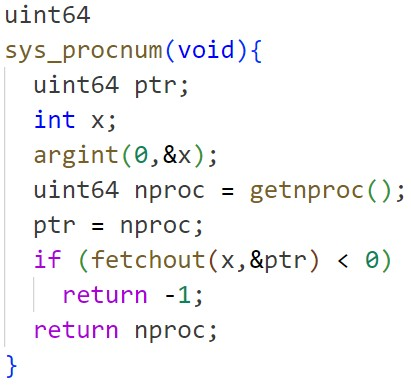
\includegraphics[width=4cm,height=4cm]{lab2-1.jpg} \label{X}}
    \hfill
    \subfloat[proc.c中]{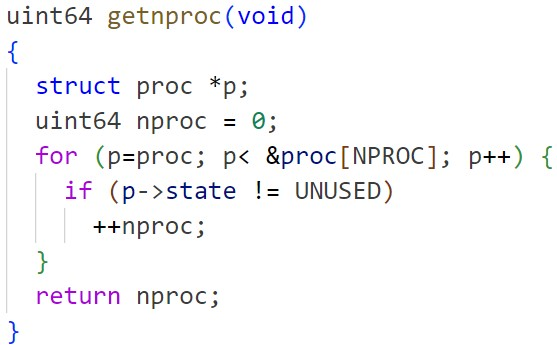
\includegraphics[width=5cm,height=4cm]{lab2-2.jpg} \label{Y}}
\end{figure*}\\
\noindent 五、运行结果:
\begin{figure}[htbp]
    \centering
    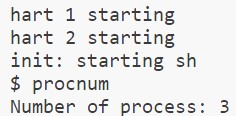
\includegraphics[width=3cm,height=2cm]{lab2-3.jpg}
\end{figure}\\
\begin{Large}
    \noindent 实验二、freemem\\
\end{Large}
\noindent 一、实现思路:\\
\hspace*{2em}在阅读了kalloc.c以及文档中的hint后,我感觉具体的实现并不复杂。主要的空闲内存存在freelist中,我们先上锁,之后统计大小即可。而作为一个list,可以很自然地用next遍历,而每次只要加上xv6自带参数PGSIZE即可。\\
\noindent 二、调用顺序:\\
\hspace*{2em}上述的思路应该在kalloc.c中新增函数,因为在sysproc.c中是没法直接调用kmem的。先在kalloc.c中增加uint64 getfreemem(void)函数,所以在def.h中增加其声明,最后由sysproc.c中的函数uint64 freemem(void)调用;以及完成了ppt中的步骤后,之后用户程序freemem.c即可正常调用。\\
\noindent 三、实验代码:
\begin{figure*}[!h]
    \centering
    \subfloat[sysproc.c中]{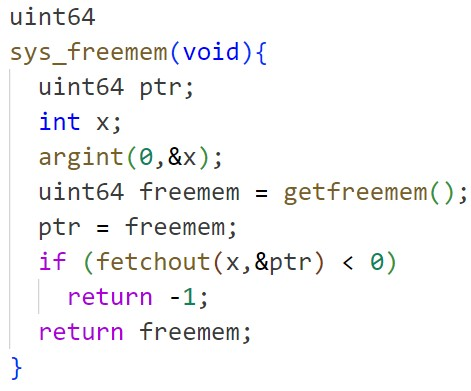
\includegraphics[width=4cm,height=4cm]{lab2-4.jpg} \label{X}}
    \hfill
    \subfloat[kalloc.c中]{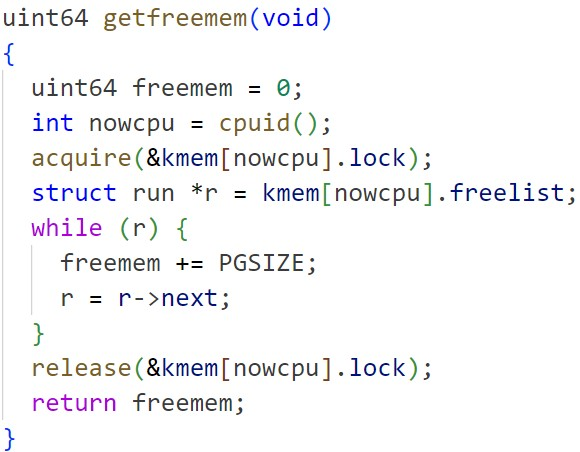
\includegraphics[width=5cm,height=4cm]{lab2-5.jpg} \label{Y}}
\end{figure*}\\
\noindent 五、运行结果:
\begin{figure}[htbp]
    \centering
    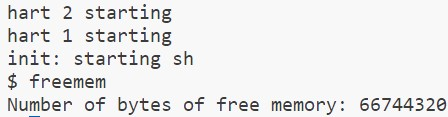
\includegraphics[width=5cm,height=2cm]{lab2-6.jpg}
\end{figure}
\newpage
\begin{Large}
    \noindent 实验三、trace\\
\end{Large}
\noindent 一、实现思路:\\
\hspace*{2em}首先,为了让系统调用被正确跟踪,需要从其掩码入手,给struct proc增加一个新的变量,int mask。之后在syscall时识别并及时打印就可以。\\
\noindent 二、具体实现:\\
\hspace*{2em}通过观察syscall.c中的syscall函数后,我们发现,syscall会获取一个num,而这个num就可以用来作掩码判断。以及还需要完善的点:sys\_trace负责获取参数,并向当前进程传递;需要考虑fork时mask也被传递,所以要在proc.c的fork函数中增添一行 np->mask = p->mask;在syscall函数中,如果直接打印syscalls[num],会出现乱码,为了解决该现象,新增一char*数组syscall\_name,如此打印就无误。\\
\noindent 三、实验代码:
\begin{figure}[htbp]
    \centering
    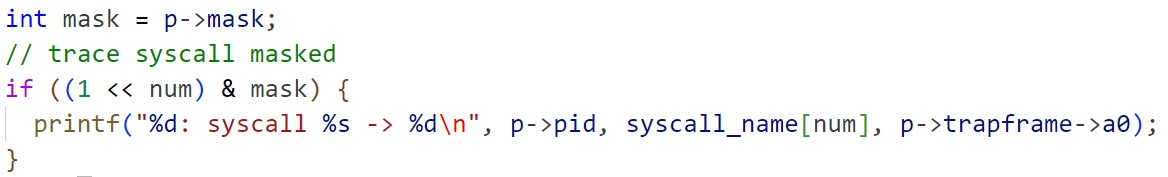
\includegraphics[width=10cm,height=2cm]{lab2-7.jpg}
\end{figure}\\
\noindent 四、运行结果:
\begin{figure}[htbp]
    \centering
    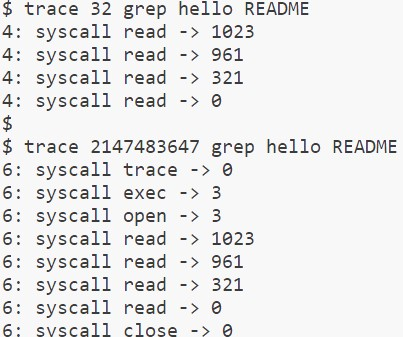
\includegraphics[width=5cm,height=5cm]{lab2-8.jpg}
\end{figure}\\
\begin{Large}
    \noindent 实验四、流程概述\\
\end{Large}
\noindent 1.系统调用过程:\\
\hspace*{2em}用户使用系统调用的接口,通过syscall函数触发系统调用;处理器从用户模式变为内核模式;在内核模式内系统选择要执行的调用;执行系统调用,可能会会从用户空间拿取数据;返回系统调用结果,返回用户模式。\\
\noindent 2.malloc的底层实现原理:\\
\hspace*{2em}查阅到的资料经概述后如下:(1)内存池初始化:在启动时,xv6会初始化一个内存池,用于存储所有可用的内存块。
(2)内存块分配:malloc 函数会调用内存分配器。内存分配器的任务是从内存池中找到足够大的空闲内存块,然后将其标记为已分配。分配器返回指向此块的指针。
(3)内存块释放:完成使用分配的内存后,可以使用 free 函数来将内存块返回给内存分配器。内存分配器会将被释放的内存块标记为可用。
(4)碎片管理:内存分配器可能需要处理内存碎片的问题。碎片是未分配的小块内存,通常由已分配内存块之间的空间导致。一些内存分配器使用合并或分割策略来最小化碎片。在xv6中,内存分配器采用首次适配策略,即它会尽量使用第一个足够大的空闲块,而不会尝试合并或分割块。
(5)内存池管理:内存分配器还需要管理内存池,以跟踪哪些块是可用的,哪些是已分配的。
\end{document}